%!TEX TS-program = xelatex
\documentclass[]{friggeri-cv}
\usepackage{afterpage}
\usepackage{color}
\usepackage{xcolor}
\usepackage{hyperref}
\hypersetup{
    pdftitle={},
    pdfauthor={},
    pdfsubject={},
    pdfkeywords={},
    colorlinks=false,       % no lik border color
   allbordercolors=white    % white border color for all
}
\addbibresource{bibliography.bib}
\RequirePackage{xcolor}
\definecolor{pblue}{HTML}{0395DE}

\begin{document}
\header{\hspace{3.0cm} Rogério Jorge }{12/04/1992}
      %{\hspace{3.0cm}Rogério Manuel Cabete de Jesus Jorge, April 12, 1992}
      
% Fake text to add separator      
\fcolorbox{white}{gray}{\parbox{\dimexpr\textwidth-2\fboxsep-2\fboxrule}{%
.....
}}

% In the aside, each new line forces a line break
\begin{aside}
  \section{Address}
    %\textbf{Switzerland}
    Route de Genève, 78 1028, Préverenges, Lausanne, Switzerland
    ~
    %\textbf{Portugal}
    %Avenida Almirante Reis, 56 1170, Lisboa, Portugal
    ~
    %Rua da Escola, nº23 2º direito, Chã-Tavarede, Figueira da Foz, Portugal
    ~
  \section{Tel}
    %+351 920520221 (PT)
    +41 0765074111 (CH)
    ~
  \section{Mail}
    %\href{mailto:rogeriodejesusjorge@gmail.com}{\textbf{rogeriodejesusjorge@}\\gmail.com}
    \href{mailto:rogerio.jorge@epfl.ch}{\textbf{rogerio.jorge@}\\epfl.ch}
    %\href{mailto:rogerio.jorge@ist.pt}{\textbf{rogerio.jorge@}\\ist.pt}
    ~
  \section{Web}
    \href{http://web.ist.utl.pt/~rogerio.jorge}{web.ist.utl.pt\\/\char`\~rogerio.jorge}
    \href{https://pt.linkedin.com/in/rogeriodejesusjorge}{pt.linkedin.com\\/in/rogeriodejesusjorge}
    %~
  %\section{Programming}
    %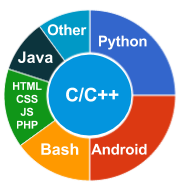
\includegraphics[scale=0.62]{img/programming.png}
    %~
  %\section{OS Preference}
    %\textbf{GNU/Linux}
\includegraphics[scale=0.40]{img/5stars.png}
    %\textbf{Unix}
\includegraphics[scale=0.40]{img/4stars.png}
    %\textbf{MacOS}
\includegraphics[scale=0.40]{img/2stars.png}
    %\textbf{Windows}
\includegraphics[scale=0.40]{img/1stars.png}
    %~
  %\section{Personal Skills}
    %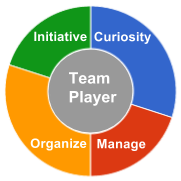
\includegraphics[scale=0.62]{img/personal.png}
    ~
  \section{Research Topics}
    %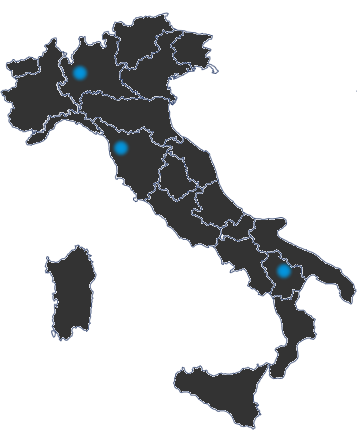
\includegraphics[scale=0.25]{img/italia.png}
    \textbf{Plasma Physics}
    Magnetic Confinement
    Tokamak Edge (SOL)
    \textbf{General Relativity}
    Black Holes
    General Relativistic MHD
    ~
  \section{Languages}
    \textbf{Portuguese}
\includegraphics[scale=0.40]{img/5stars.png}
    \textbf{English}
\includegraphics[scale=0.40]{img/4stars.png}
    \textbf{French}
\includegraphics[scale=0.40]{img/3stars.png}
    Matlab/Mathematica
    Latex/Fortran/Linux
    HTML/CSS/PHP/MySQL
\end{aside}

\section{Experience}
\begin{entrylist}
  \entry
    {01/15 - Now}
    {PhD Student}
    {\\
    Swiss Plasma Center (SPC) - EPFL, Lausanne Switzerland
    \\
    Instituto de Plasmas e Fusão Nuclear (IPFN), APPLAuSE - IST, Lisboa Portugal}
    {Plasma physics theory and modelling with applications to nuclear fusion.\\ \textbf{Thesis:} \emph{"Analytical Model for the Scrape-off Layer Plasma Dynamics at Arbitrary Collisionality"}\\}
  \entry
    {08/14 - Now}
    {Startup Co-founder \& Web Developer}
    {Portal da Sabedoria}
    {Online platform to match student and tutors according to their own schedule.
    \\
    NovaBase's Gameshifters 2014 winners: start-up 24h contest, 4000€ prize
    \\
    University of Lisbon award: 2014/2015, 5000€ prize
    \\
    %Santander Totta 2015: development of online educational videos on calculus
    %\\
    \href{http://portaldasabedoria.pt}{\textbf{portaldasabedoria.pt}}
    ~
    \href{http://youtube.com/user/matmania1}{\textbf{youtube.com/user/matmania1}}\\}
\end{entrylist}

\section{Education}
\begin{entrylist}
  \entry
    {2010 - 2014}
    {Master's in Engineering Physics (18/20)}
    {Técnico Lisboa (IST), Portugal}
    {Main subjects: Nuclear Fusion, Kinetic Theory, Advanced Topics in Particle Physics, Astrophysics and Particle Physics, Topics in General Relativity.\\
    \textbf{Erasmus student} for 6 months at EPFL, Switzerland\\
    \textbf{Thesis:} \emph{"Simulation of Plasma Blobs in Realistic Tokamak Geometry",}
    \emph{Advisors: Prof. Nuno Loureiro, Prof. Paolo Ricci.}\\}
    \entry
    {2002 - 2010}
    {Classical Guitar and Music Theory Course - Music School (18/20)\hspace{1cm}}
    {Conservatório de Música David de Sousa, Figueira da Foz, Portugal}
    {Main subjects: Acoustics, Composition, Music Theory, Music History
    \\
    Winner of the 2008 International Guitar Contest of Fundão, Portugal}
\end{entrylist}

\section{Academia}
\begin{entrylist}
  \entry{2016-Now}
    {Lecture Assistant}
    {EPFL, Portugal}
    {General Physics I and II, 1st and 2nd semester Mechanical Engineering
    \\
    Advanced Physics I, 1st semester Physics}
  \entry
    {2017-Now}
    {Physics PhD Student Representative}
    {EPFL, Switzerland}
    {\emph{EPFL Doctoral Program in Physics (EDPY)}}
  \entry{2015-2016}
    {Lecture Assistant}
    {IST, Portugal}
    {Mechanics and Waves, 1st semester Engineering Physics}
  \entry
    {2010-2012}
    {Engineering Physics Class Delegate}
    {IST, Portugal}
    {\emph{}}
\end{entrylist}

\section{Main Publications}
\begin{entrylist}
  \entry
    {2016}
    {R. Jorge, P. Ricci, F. Halpern, N. Loureiro, C. Silva}
    {Physics of Plasmas 23, 10}
    {Plasma Turbulence in the Scrape-off Layer of the ISTTOK Tokamak}
  \entry
    {2015}
    {R. Jorge, E. Oliveira, J. Rocha}
    {Classical and Quantum Gravity 32, 6}
    {Greybody factors for rotating black holes in higher dimensions}
  \entry
    {2014}
    {G. Cardoso, R. Jorge, S. Nampuri}
    {Journal of High Energy Physics 2, 19}
    {Indefinite theta functions and black hole partition functions}
\end{entrylist}

\section{Conferences}
\begin{entrylist}
  \entry
    {10/2017}
    {European Fusion Theory Conference, Athens}
    {Invited Talk}
    {\emph{An analytical model for SOL plasma dynamics at arbitrary collisionality}}
  \entry
    {07/2016}
    {21st Joint EU-US Transport Task Force Meeting, Leysin}
    {Poster Presentation}
    {\emph{A Drift-Kinetic Model for Tokamak SOL Plasmas}}
\end{entrylist}

\section{Students}
\begin{entrylist}
  \entry
    {2016-2017}
    {Master's Thesis}
    {EPFL}
    {\vspace{-0.4cm}
    \begin{itemize}
    \item Sonia Gamba, Politecnico de Milano, 2017: \emph{"Analysis of Linear Instabilities in the Scrape-off Layer of a Tokamak Plasma through a Reduced Drift-Kinetic Model"}
    \end{itemize}
    }
  \entry
    {}
    {Travaux Pratique de Physique IV}
    {EPFL}
    {\vspace{-0.4cm}
    \begin{itemize}
    \item Antoine Baillod, 2017: \emph{"Gyrokinetic Equations for Scrape-off Layer Plasmas"}
    \end{itemize}
    }
  \entry
    {}
    {Summer Internship}
    {EPFL and IST}
    {\vspace{-0.4cm}
    \begin{itemize}
        \item Lorenzo Perrone, EPFL, 2017: \emph{"Parallel and Perpendicular Moment Description of Scrape-off Layer Linear Instabilities"}
        \item Konovets Vyacheslav, EPFL, 2017: \emph{"Modelling of Coulomb Collision Full-F Moment Description"}
        \item Nuno Teixeira, IST, 2017: \emph{"Convergence Studies of a Moment Pitch Angle Description of a Colisionless Plasma"}
        \item Clara Pereira, IST, 2016: \emph{"Magnetic Field Generation in Charged and Rotating Accretion Disks"}
    \end{itemize}
    }
\end{entrylist}



%\\
%\begin{flushleft}
%\emph{January 14th, 2014}
%\end{flushleft}
%\begin{flushright}
%\emph{Carmine Benedetto}
%\end{flushright}
%
%%% This piece of code has been commented by Karol Kozioł due to biblatex errors. 
% 
%\printbibsection{article}{article in peer-reviewed journal}
%\begin{refsection}
%  \nocite{*}
%  \printbibliography[sorting=chronological, type=inproceedings, title={international peer-reviewed conferences/proceedings}, notkeyword={france}, heading=subbibliography]
%\end{refsection}
%\begin{refsection}
%  \nocite{*}
%  \printbibliography[sorting=chronological, type=inproceedings, title={local peer-reviewed conferences/proceedings}, keyword={france}, heading=subbibliography]
%\end{refsection}
%\printbibsection{misc}{other publications}
%\printbibsection{report}{research reports}
%
\end{document}
